%% Sample chapter file, for use in a thesis.
%% Don't forget to put the \chapter{...} header onto each file.

\chapter{Description of the work undertaken}
\bibliography{thesis}
	\section{Discover}
	
During the discovery phase of the project the objective was to become familiar with the CEC environment, i.e. find out what tools are available and how they are being used and gather information about how to best contribute to the organisation. This was to be done while staying as open as possible, allowing any influences or ideas.

At the beginning of the project I had no knowledge about the operations within the Council or which departments would be involved. Some of the questions I wanted to answer included:
\begin{itemize}
\item Are there any activities in the Council similar to the scope of the project (or were there any in the past)?
\item Who would benefit from it and how to give those stakeholders an opportunity to be involved?
\item What questions (in terms of “channel shift”) are not answered in the Council?
At what level of abstraction should the analysis be conducted?
\item What IT systems/tools can be used in the project?
\item Who has the necessary understanding of the infrastructure and activities on the architectural level?
\item What else do I not know?
\end{itemize}

		\subsection{Meetings at the Council}
		
Initially the contact person from the Council was Sally Kerr. In response to my questions she arranged a meeting with an enterprise architect Neil Dumbleton. The purpose of the meeting was to give me an opportunity to ask questions regarding organisational structure as well as context of the project.

As it turned out, it was a first meeting in a series. There was no formalised documentation or central place with knowledge about on-going projects that was made available to the author. As a result, personal meetings were the only way to understand activity in the Council. Moreover, it was only thanks to good will of many employees at the City of Edinburgh Council that this was possible.

The diagram below shows all the people who I interacted with during the entire project. Connections between different actors represent how I got to know them. Circles with coloured backgrounds highlight people who I spoke with in this phase. Orange colour marks people related with University of Edinburgh, blue is for CEC employees. Level of a circle does not reflect a position in the Council’s structure - it is used solely for increasing legibility of the diagram.

\begin{figure}[h]
\centering
     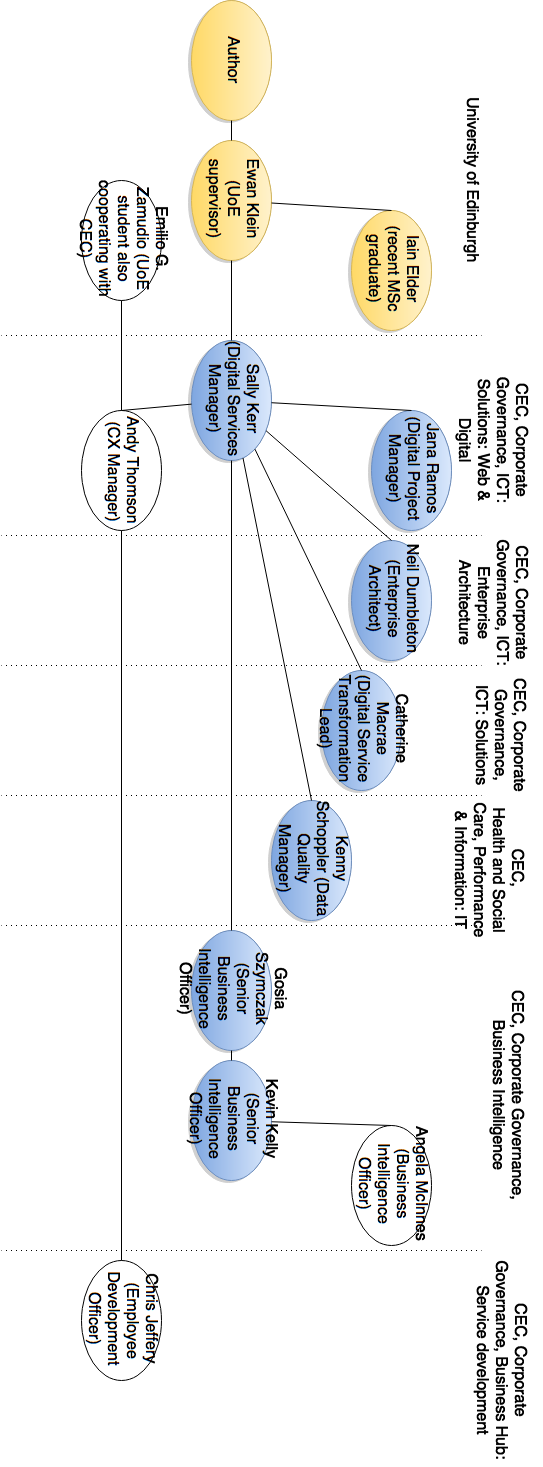
\includegraphics[angle=270, height=\textheight]{Discovery_phase_people.png}
      \caption{CEC employees involved in the project.}
       \label{normal_case}
\end{figure}
		
		\subsection{CRM data}
		
		\subsection{Mosaic UK Consumer and Demographic data}
		
		\subsection{IBM Cognos}
		
			\subsubsection{Introduction}
			
			\subsubsection{Working with IBM Cognos BI}

	\section{Define}

	\section{Develop}
	
	\section{Deliver}